\documentclass{article}

\usepackage{fancyhdr}
\usepackage{extramarks}
\usepackage{amsmath}
\usepackage{amsthm}
\usepackage{amsfonts}
\usepackage{tikz}
\usepackage[plain]{algorithm}
\usepackage{algpseudocode}
\usepackage{amssymb}



\usetikzlibrary{automata,positioning}

%
% Basic Document Settings
%

\topmargin=-0.45in
\evensidemargin=0in
\oddsidemargin=0in
\textwidth=6.5in
\textheight=9.0in
\headsep=0.25in

\linespread{1.1}

\pagestyle{fancy}
\lhead{\hmwkAuthorName}
\chead{\hmwkClass\ (\hmwkClassInstructor\ \hmwkClassTime): \hmwkTitle}
\rhead{\firstxmark}
\lfoot{\lastxmark}
\cfoot{\thepage}

\renewcommand\headrulewidth{0.4pt}
\renewcommand\footrulewidth{0.4pt}

\setlength\parindent{0pt}

%
% Create Problem Sections
%

\newcommand{\enterProblemHeader}[1]{
    \nobreak\extramarks{}{Problem \arabic{#1} continued on next page\ldots}\nobreak{}
    \nobreak\extramarks{Problem \arabic{#1} (continued)}{Problem \arabic{#1} continued on next page\ldots}\nobreak{}
}

\newcommand{\exitProblemHeader}[1]{
    \nobreak\extramarks{Problem \arabic{#1} (continued)}{Problem \arabic{#1} continued on next page\ldots}\nobreak{}
    \stepcounter{#1}
    \nobreak\extramarks{Problem \arabic{#1}}{}\nobreak{}
}

\setcounter{secnumdepth}{0}
\newcounter{partCounter}
\newcounter{homeworkProblemCounter}
\setcounter{homeworkProblemCounter}{1}
\nobreak\extramarks{Problem \arabic{homeworkProblemCounter}}{}\nobreak{}

%
% Homework Problem Environment
%
% This environment takes an optional argument. When given, it will adjust the
% problem counter. This is useful for when the problems given for your
% assignment aren't sequential. See the last 3 problems of this template for an
% example.
%
\newenvironment{homeworkProblem}[1][-1]{
    \ifnum#1>0
        \setcounter{homeworkProblemCounter}{#1}
    \fi
    \section{Problem \arabic{homeworkProblemCounter}}
    \setcounter{partCounter}{1}
    \enterProblemHeader{homeworkProblemCounter}
}{
    \exitProblemHeader{homeworkProblemCounter}
}

%
% Homework Details
%   - Title
%   - Due date
%   - Class
%   - Section/Time
%   - Instructor
%   - Author
%

\newcommand{\hmwkTitle}{Homework\ \#3}
\newcommand{\hmwkDueDate}{January 31st, 2017}
\newcommand{\hmwkClass}{Elements of Algebra I}
\newcommand{\hmwkClassTime}{Section 161}
\newcommand{\hmwkClassInstructor}{Professor Deepam Patel}
\newcommand{\hmwkAuthorName}{Yao Xiao}

%
% Title Page
%

\title{
    \vspace{2in}
    \textmd{\textbf{\hmwkClass:\ \hmwkTitle}}\\
    \normalsize\vspace{0.1in}\small{Due\ on\ \hmwkDueDate\  }\\
    \vspace{0.1in}\large{\textit{\hmwkClassInstructor\ \hmwkClassTime}}
    \vspace{3in}
}

\author{\textbf{\hmwkAuthorName}}
\date{}

\renewcommand{\part}[1]{\textbf{\large Part \Alph{partCounter}}\stepcounter{partCounter}\\}

%
% Various Helper Commands
%

% Useful for algorithms
\newcommand{\alg}[1]{\textsc{\bfseries \footnotesize #1}}

% For derivatives
\newcommand{\deriv}[1]{\frac{\mathrm{d}}{\mathrm{d}x} (#1)}

% For partial derivatives
\newcommand{\pderiv}[2]{\frac{\partial}{\partial #1} (#2)}

% Integral dx
\newcommand{\dx}{\mathrm{d}x}

% Alias for the Solution section header
\newcommand{\solution}{\textbf{\large Solution}}

% Probability commands: Expectation, Variance, Covariance, Bias
\newcommand{\E}{\mathrm{E}}
\newcommand{\Var}{\mathrm{Var}}
\newcommand{\Cov}{\mathrm{Cov}}
\newcommand{\Bias}{\mathrm{Bias}}

\begin{document}

\maketitle

\pagebreak

\begin{homeworkProblem}
\subsection{1)}
1. Not commutative, when \(x=1 \ y=0\), \(x*y=1 \ y*x=0\) \\
2. Not associative, when \[
(x+2y+xy)+2z+(x+2y+xy)z=x + 2 y + x y + 2 z + x z + 2 y z + x y z
\]
\[
x+2(y+2z+yz)+x(y+2z+yz)=x+2y+z4+2yz+xy+2xz+xyz
\]
3. There's no identity due to 0*y \(\neq\) x*0 and 2y \(\neq\) y\\
4. There's no inverse due to 3
\subsection{2)}
1. It's commutative, since when \(x>y \ |x-y|=x-y\ |y-x|=-(y-x)=x-y\)
when \(y>x \ |y-x|=y-x \ |x-y|=-(x-y)=y-x\) \\
2. It's not associative, when x=2,y=1,z=1
\[
||2-1|-1|=0 
\]
while
\[
|2-|1-1||=2
\]
3. There's no identity since when \(x<0\), the result must be positive so there would be no e satisfied \\
4. There's no inverse due to 3
\subsection{3)}
1. It's commutative since \(max{x,y}=max{y,x}\)\\
2. It's associative since \(max(x, max(y, z))
= max(x, y, z) = max(max(x, y), z)\)\\
3. There's no identity, If \(e \in \mathbb{R}\) were an identity, then we can choose an integer \(x < e\) and for this integer and we could get \(max(x,e)=e\neq\ x\). So there's no identity\\
4. There's no inverse due to 3


\end{homeworkProblem}

\begin{homeworkProblem}
\[
\begin{split}
g \in G\\
e &= g^{-1} * g\\
(g^{-1})^{-1}*e &=(g^{-1})^{-1} * (g^{-1} * g)\\
 &=((g^{-1})^{-1} * g^{-1}) * g)\\
\end{split}
\]
Since \(g^{-1}*g=e\) Let \(g'=g^{-1}\) \(g'^{-1}*g'=e\)
So the formula above becomes
\[
\begin{split}
(g^{-1})^{-1}*e&=(e) * g)\\
(g^{-1})^{-1}&=g
\end{split}
\]
In order to show \((gh)^{-1}=h^{-1}g^{-1}\)
We just need to show the right hand side is the inverse of \(gh\).
\[\begin{split}
	gh(h^{-1}g^{-1})=g(h^{-1}h)g^{-1}\\
	&=geg^{-1}\\
	&=gg^{-1}\\
	&=e
\end{split}\]
So \((h^{-1}g^{-1})\) is the inverse of gh, as a result, \(gh^{-1}=h^{-1}g^{-1}\)
\end{homeworkProblem}

\begin{homeworkProblem}
Using the theory of Problem 2, we could get
\[\begin{split}
g^{-1}h^{-1}&=(hg)^{-1}\\
&=(gh)^{-1}\\
&=h^{-1}g^{-1}
\end{split}\]
So its inverse commutes as well.
\end{homeworkProblem}

\begin{homeworkProblem}
By Problem 2, we have
\[\begin{split}
(ab)^{-1}=b^{-1}a^{-1}=a^{-1}b^{-1}
\end{split}\]
If it commutes\\
So we could get 
\[\begin{split}
(ab)^n=((ab)^{-1})^{-n}=(a^{-1}b^{-1})^{-n}=a^nb^n
\end{split}\]

\end{homeworkProblem}

\begin{homeworkProblem}
\begin{enumerate}
\item Closure. By the definition, If \( x,y\in  G\)
\[
\exists x^{-1}, y^{-1} \in S
\]
From problem 2, we know \(y^{-1}*x^{-1}=(xy)^{-1}\). If xy has an inverse, so it must be in G. We proved that \( x*y \in G\)
\item Associative, since G is a subset of S and S , it must hold
\item Identity, since \(e \in S\) , e has an inverse e, \(e \in G\) must hold
\item Inverse, let \( x \in G\), there must be an inverse \( x^{-1} \in S\) since \(x \in S\). We know that \( (x^{-1})^{-1}=x \) and \( x \in G\). There must be an element \( x^{-1} \in G\)

\end{enumerate}
\end{homeworkProblem}

\begin{homeworkProblem}
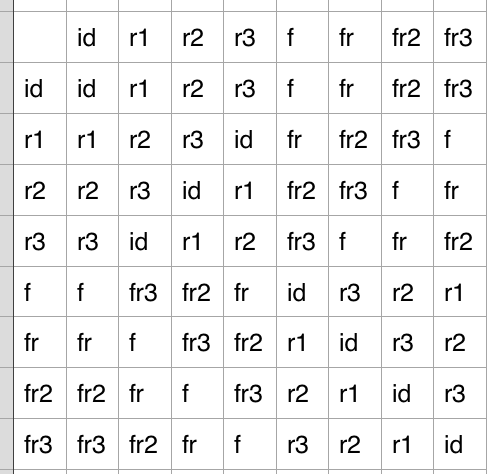
\includegraphics[scale=1]{table.png} 
\end{homeworkProblem}

\begin{homeworkProblem}
We assume set \(\mathbb{Z}_n\), which 2 has an inverse. So \( \exists k,l \in \mathbb{Z}_n \) such that \(2k+1=nl \) so \(2k=nl-1\) , nl-1 is even, nl must be odd, which means n and l must be odd. n is odd.
\end{homeworkProblem}

\begin{homeworkProblem}
(12)(13) doesn't commute. (12)(13)=(132). (13)(12)=(123)
\end{homeworkProblem}


\end{document}
